%%%%%%%%%%%%%%%%%%%%%%%%%%%%%%%%%%%%%%%%%
% Dreuw & Deselaer's Poster
% LaTeX Template
% Version 1.0 (11/04/13)
%
% Created by:
% Philippe Dreuw and Thomas Deselaers
% http://www-i6.informatik.rwth-aachen.de/~dreuw/latexbeamerposter.php
%
% This template has been downloaded from:
% http://www.LaTeXTemplates.com
%
% Edited by: Manfred Brill
%
% License:
% CC BY-NC-SA 3.0 (http://creativecommons.org/licenses/by-nc-sa/3.0/)
%%%%%%%%%%%%%%%%%%%%%%%%%%%%%%%%%%%%%%%%%

% ----------------------------------------------------------------------------------------
%  Kopf- und Fusszeile werden in beamertheme16pd2.sty definiert!
% ----------------------------------------------------------------------------------------

%----------------------------------------------------------------------------------------
%   PACKAGES AND OTHER DOCUMENT CONFIGURATIONS
%----------------------------------------------------------------------------------------
\documentclass[final,hyperref={pdfpagelabels=false}]{beamer}

\usepackage{todo}

\usepackage{wrapfig}

\usepackage[orientation=portrait, size=a0, scale=1.4]{beamerposter}

\usetheme{I6pd2} % Use the I6pd2 theme supplied with this template

\usepackage[german]{babel}
%\usepackage[english]{babel} % English language/hyphenation

\usepackage{amsmath,amsthm,amssymb,latexsym}

%\usepackage{times}\usefonttheme{professionalfonts}  % Uncomment to use Times as the main font
%\usefonttheme[onlymath]{serif} % Uncomment to use a Serif font within math environments

\boldmath % Use bold for everything within the math environment

\usepackage{booktabs} % Top and bottom rules for tables

\usepackage{multicol}

\newcommand{\imagePath}{./figures}

\graphicspath{{figures/}} % Location of the graphics files

\usecaptiontemplate{\small\structure{\insertcaptionname~\insertcaptionnumber: }\insertcaption}
 % A fix for figure numbering

%----------------------------------------------------------------------------------------
%   TITLE SECTION
%----------------------------------------------------------------------------------------

\title{\huge Virtual Science Lab}

\author{Manfred Brill, Marc Zintel, Philipp Lauer}

\institute{Department of Computer Science and Microsystems Technology}
%----------------------------------------------------------------------------------------

\begin{document}

\addtobeamertemplate{block end}{}{\vspace*{2ex}} % White space under blocks

\begin{frame}[t] % The whole poster is enclosed in one beamer frame

\begin{columns}[t] % The whole poster consists of two major columns, each of which can be subdivided further with another \begin{columns} block - the [t] argument aligns each column's content to the top

\begin{column}{.02\textwidth}\end{column} % Empty spacer column

\begin{column}{.465\textwidth} % The first column


\begin{block}{Virtual Reality}
    \begin{figure}
    	\centering
    	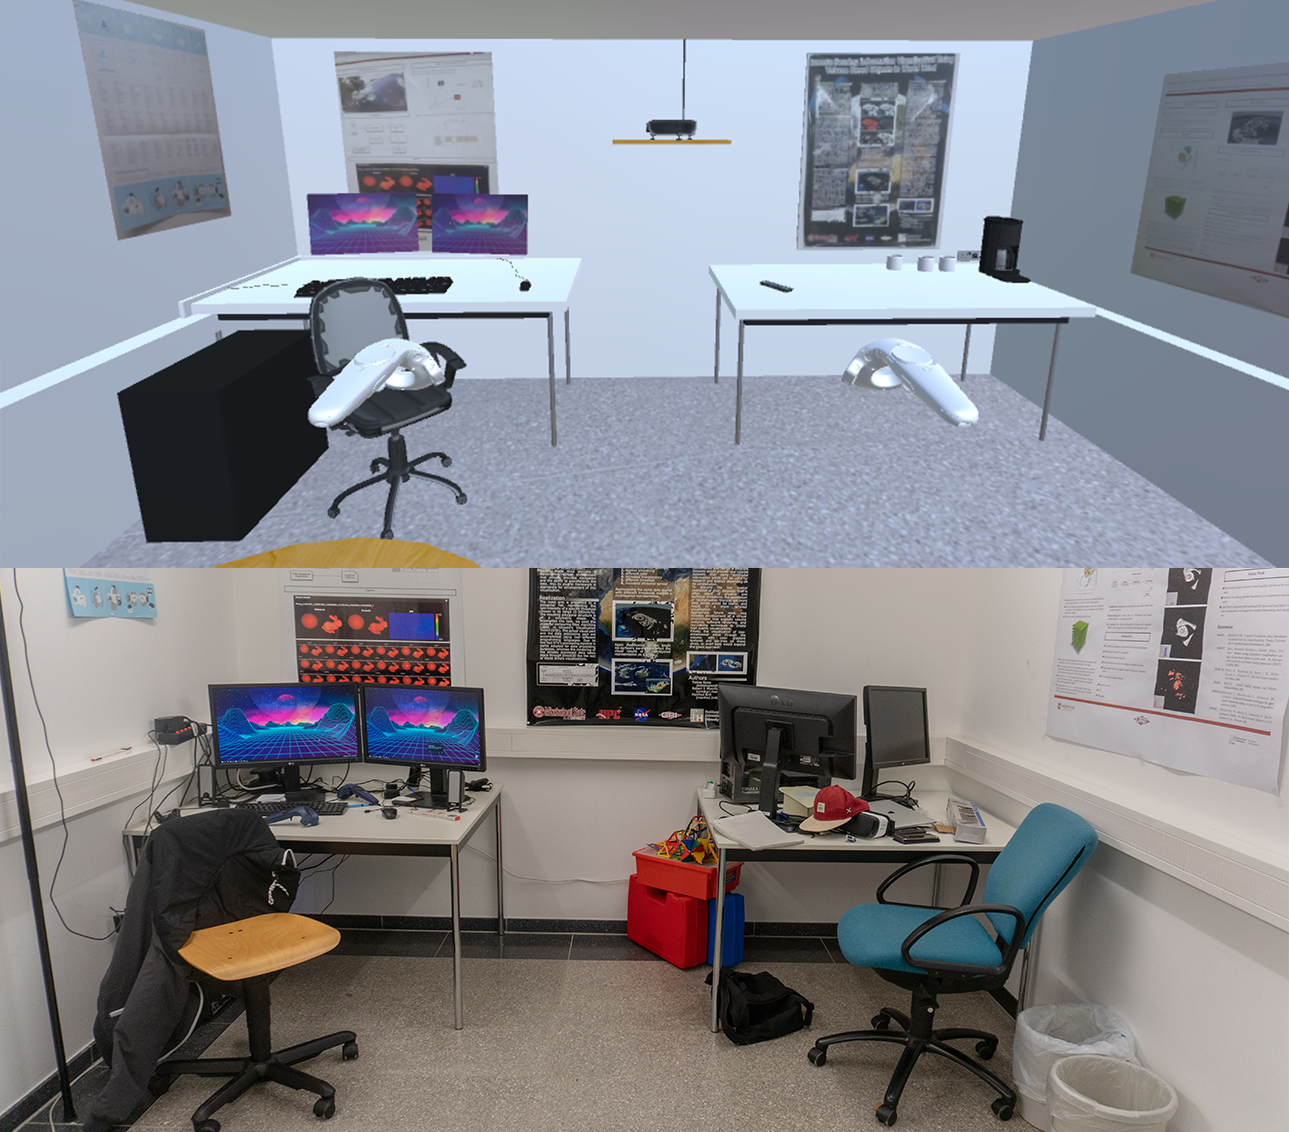
\includegraphics[width=0.95\linewidth]{labor_vgl}

    \end{figure}
    
    \vspace{20px}
\end{block}

\vspace{0.3cm}

\begin{block}{Dijkstra}
	\begin{figure}
		\centering
		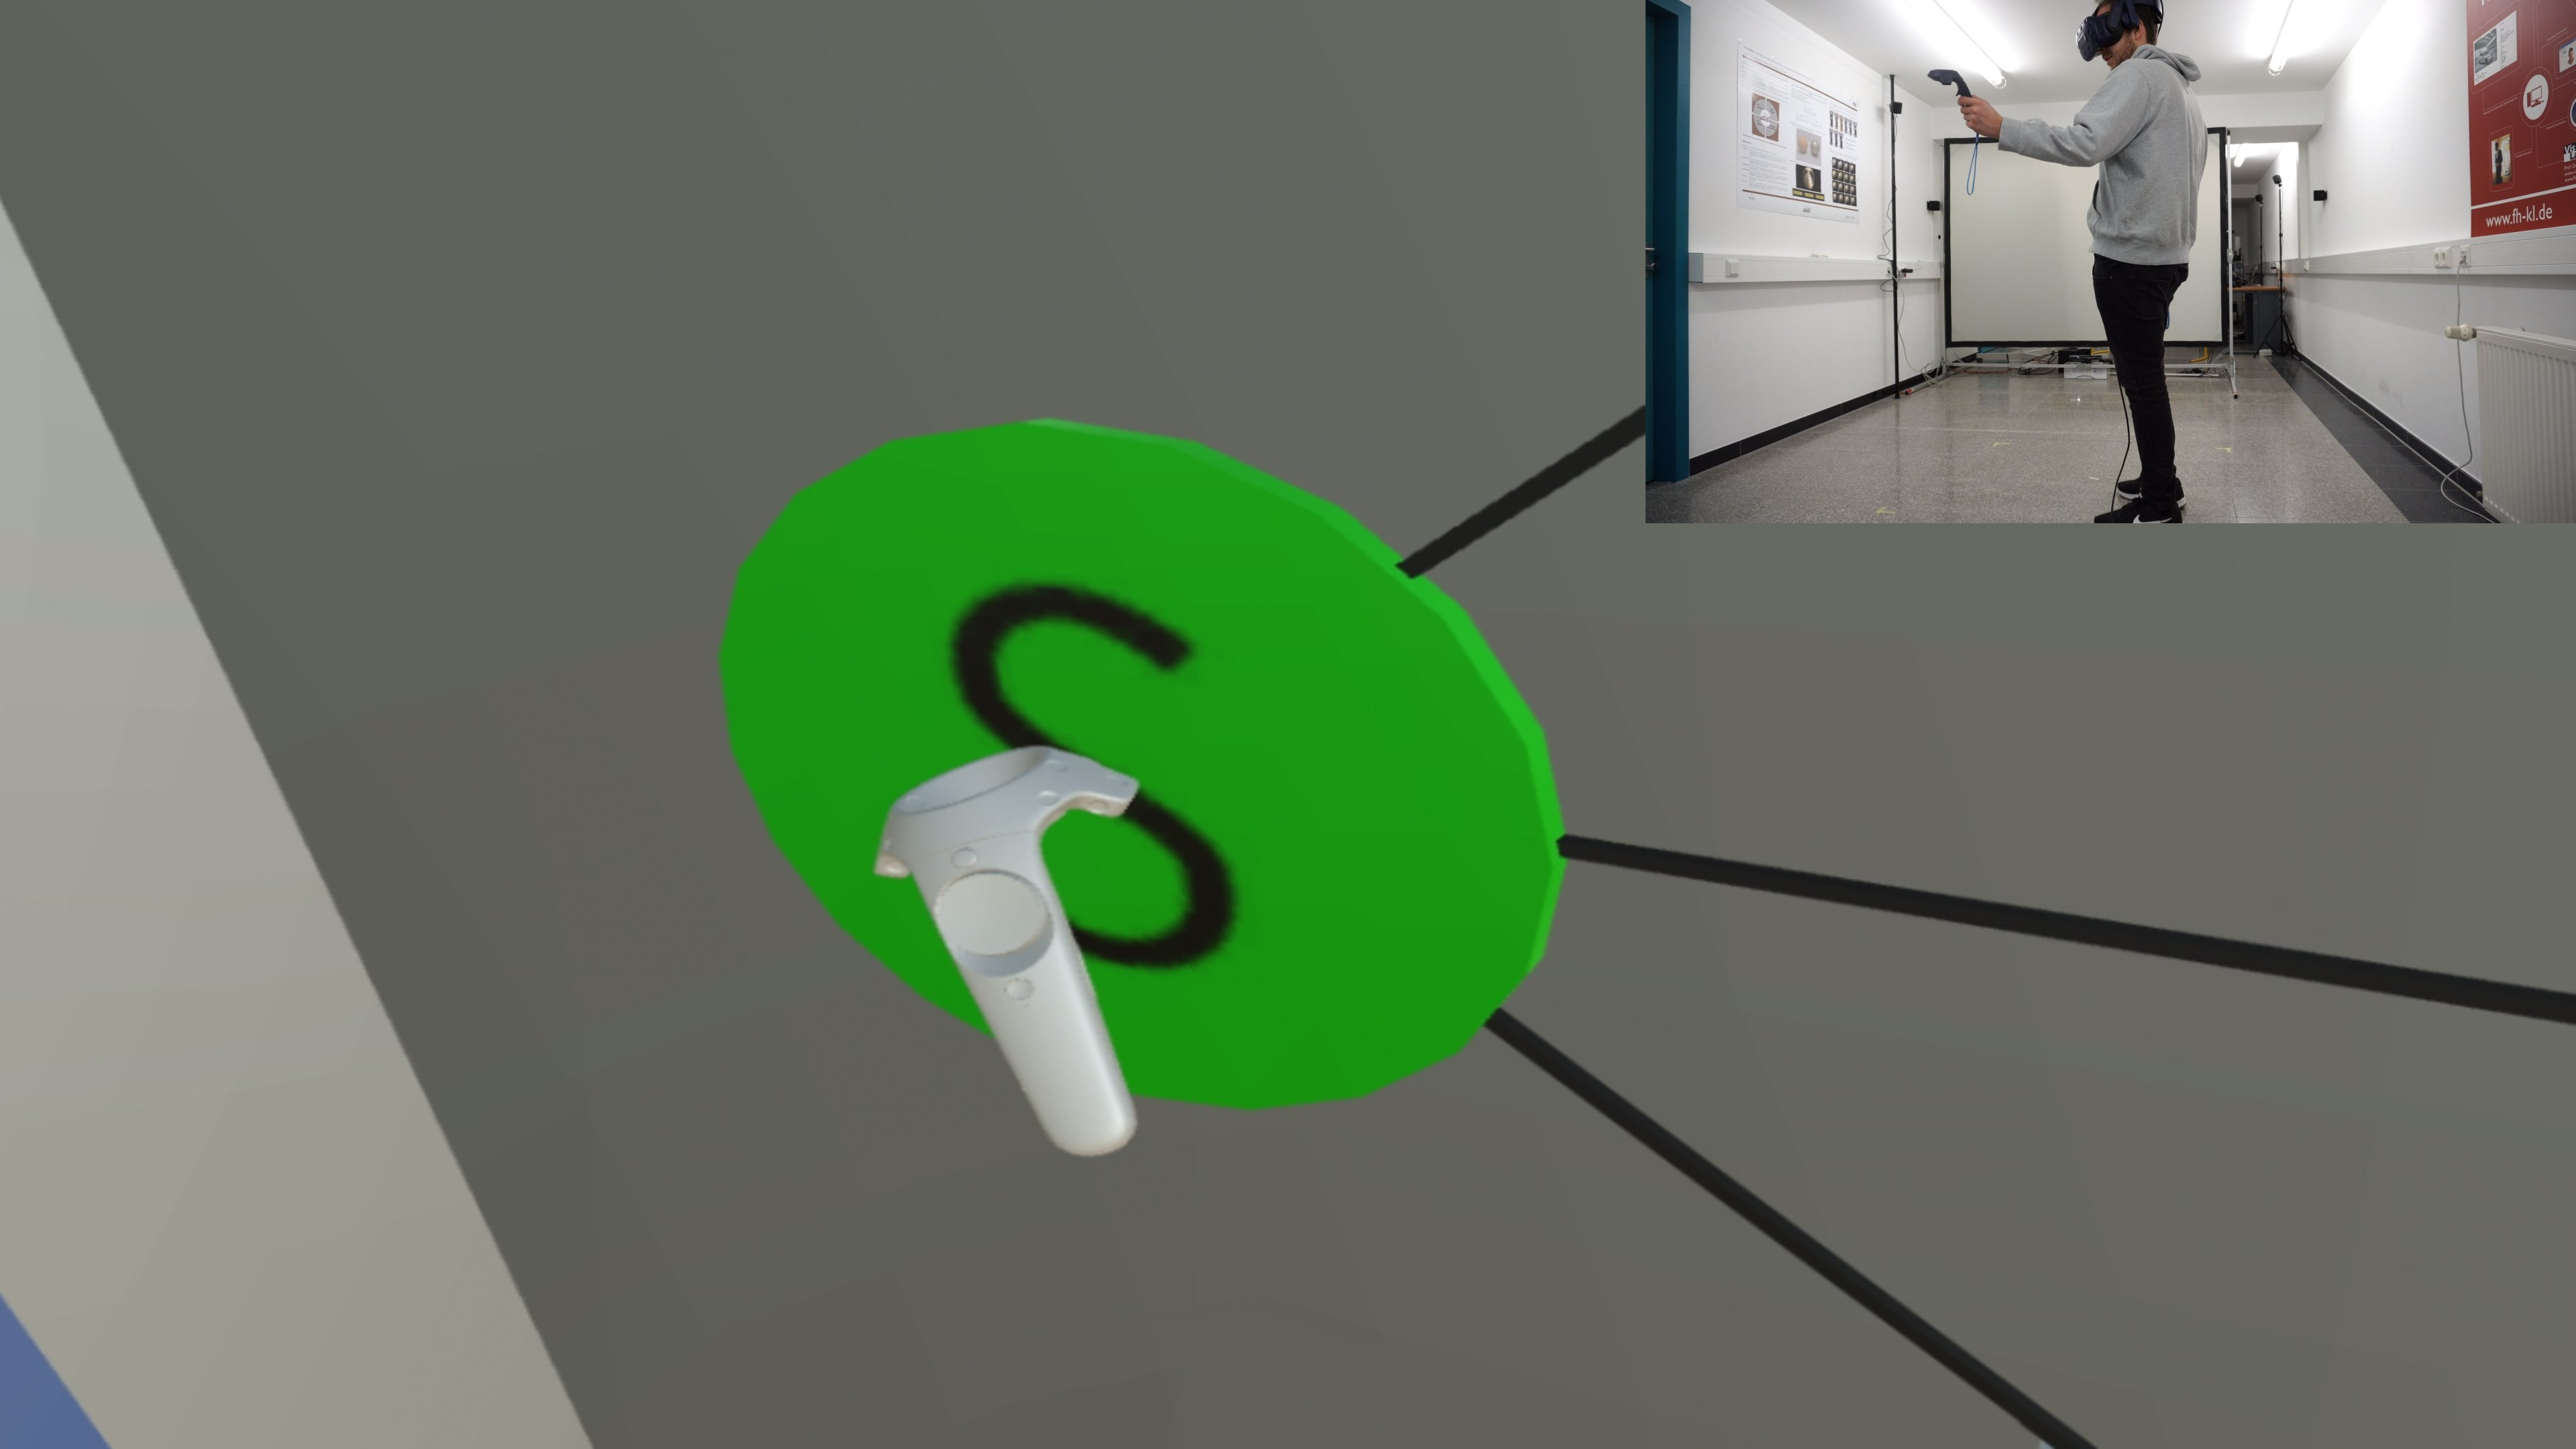
\includegraphics[width=0.95\linewidth]{VSL_Screen_2}

	\end{figure}
\end{block}

\vspace{0.3cm}

\begin{block}{Chemistry}
    \begin{figure}
    	\centering
    	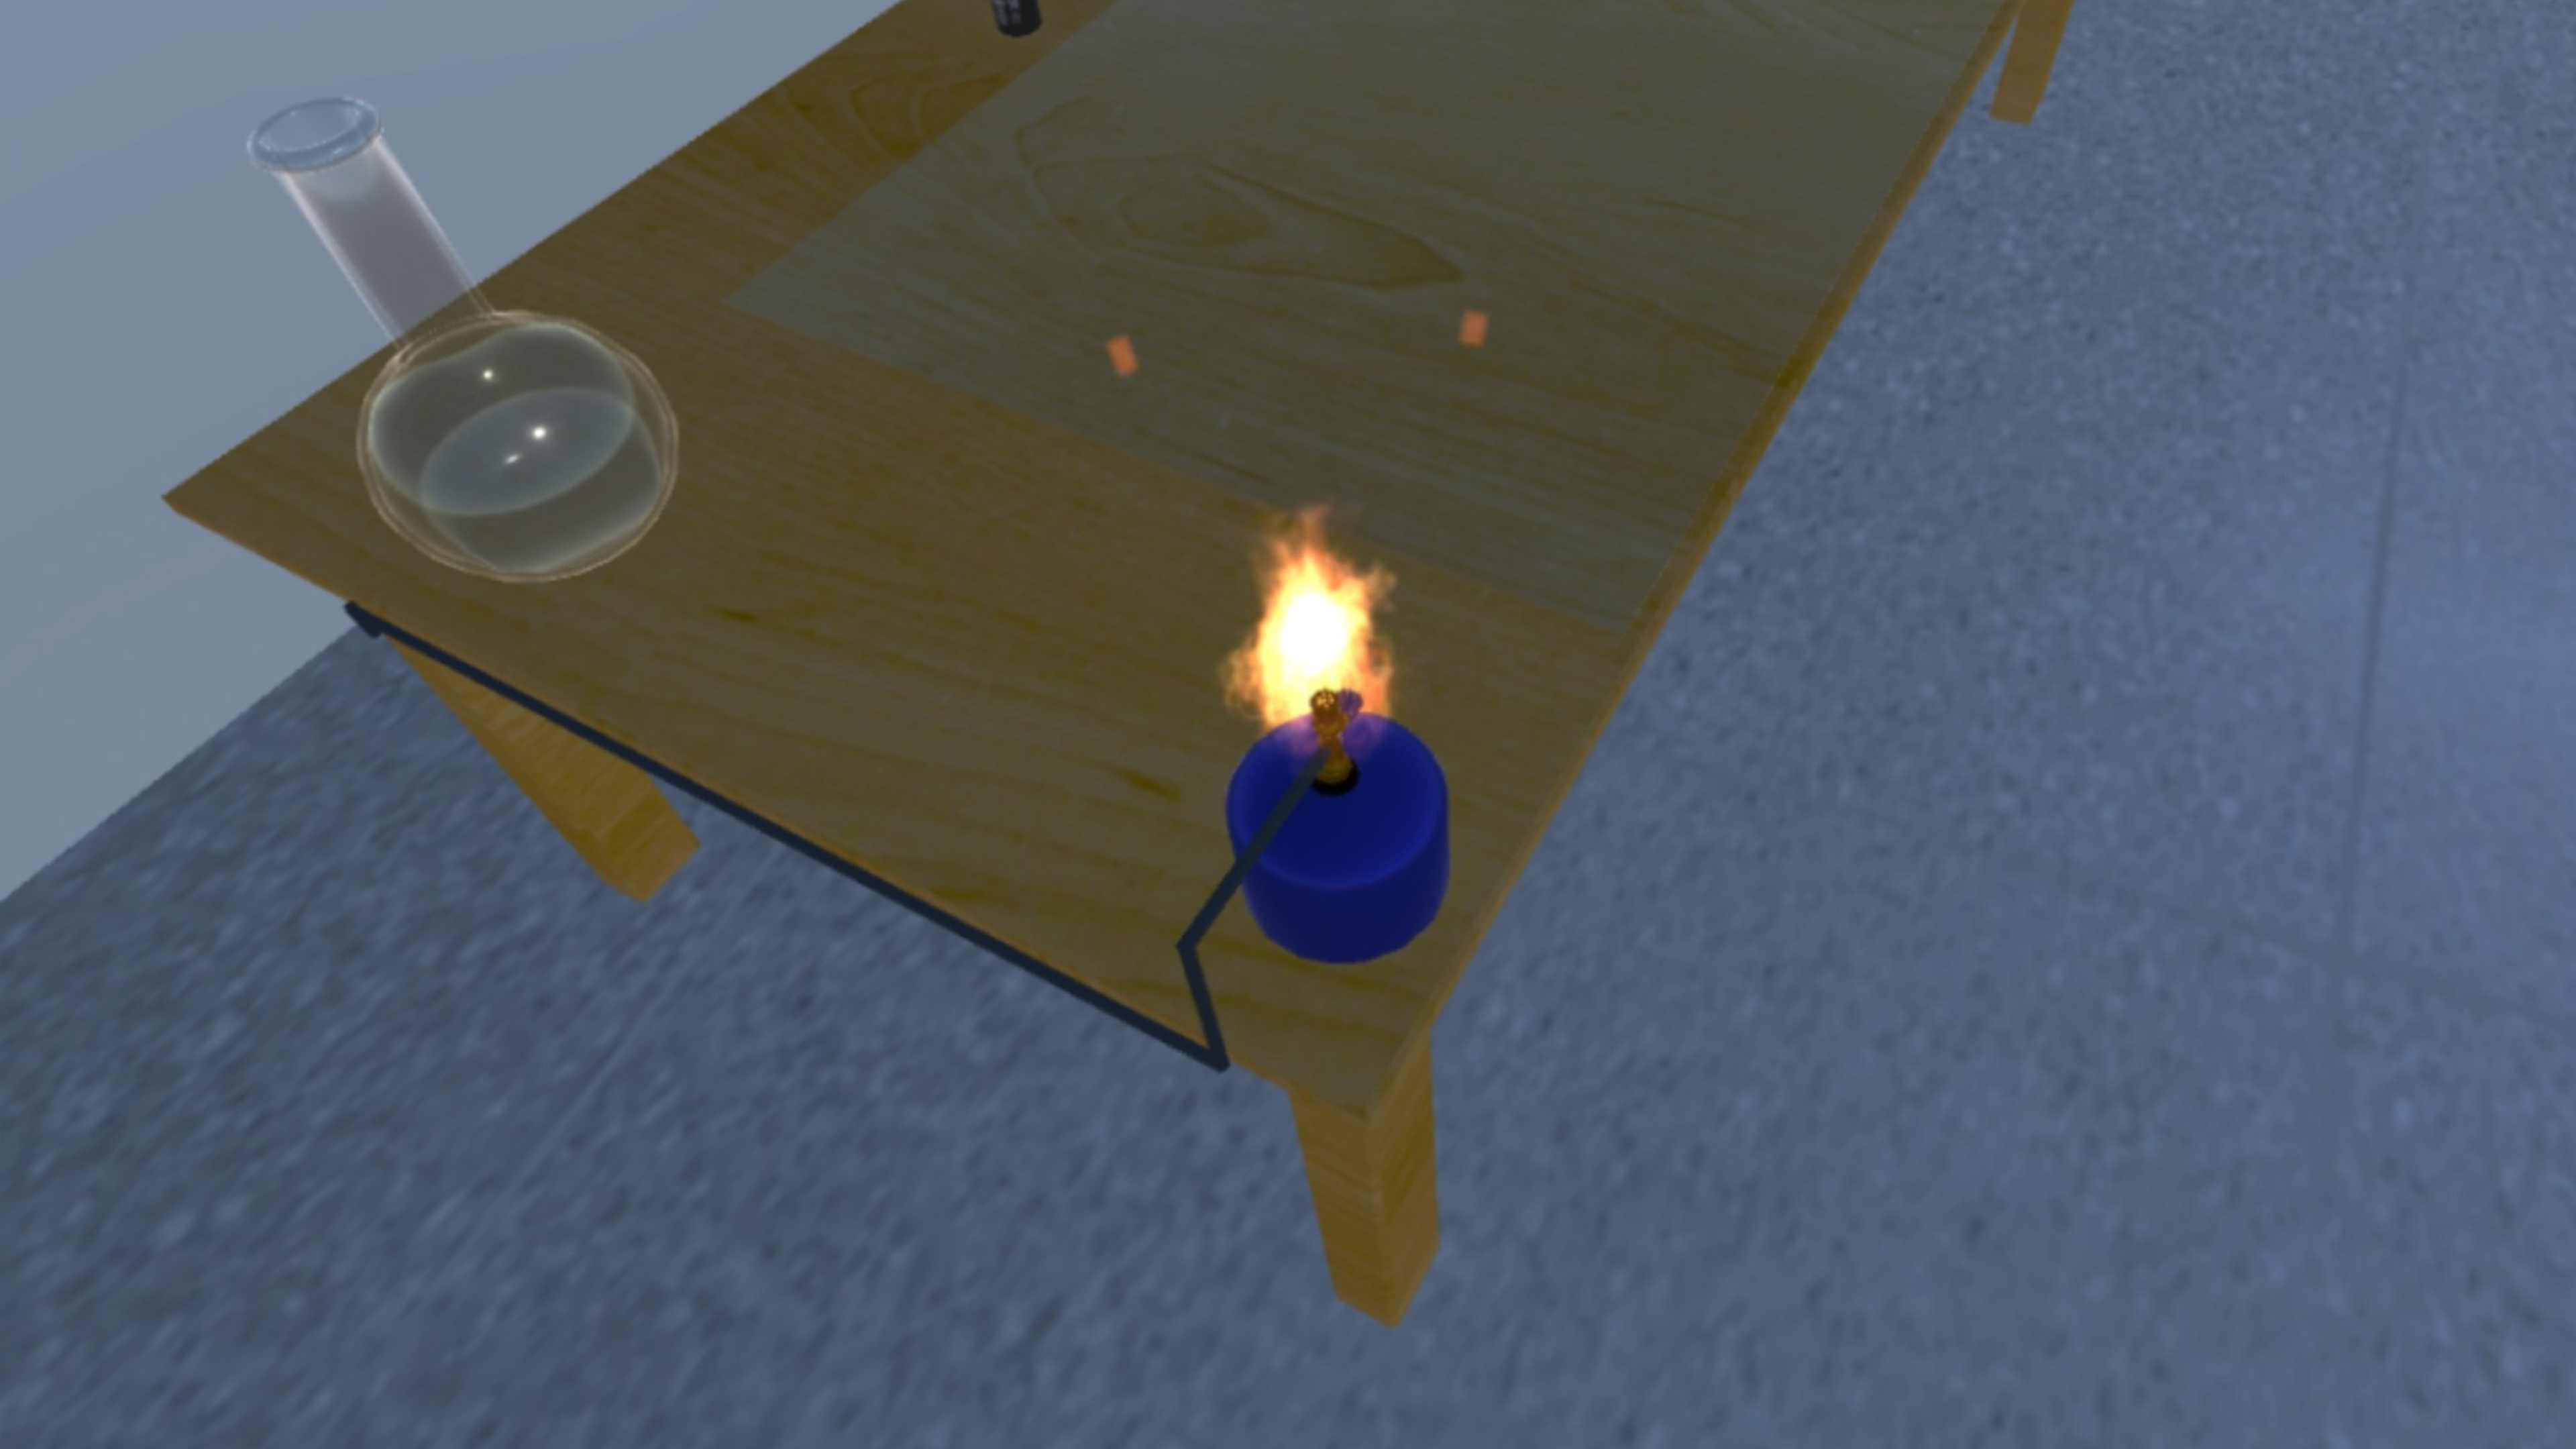
\includegraphics[width=0.95\linewidth]{bunsenbrenner}
    \end{figure}
\end{block}
%----------------------------------------------------------------------------------------

\end{column} % End of the first column

\begin{column}{.03\textwidth}\end{column} % Empty spacer column

\begin{column}{.465\textwidth} % The second column

\begin{block}{Elektrotechnik}
	
	\begin{figure}
		\centering
		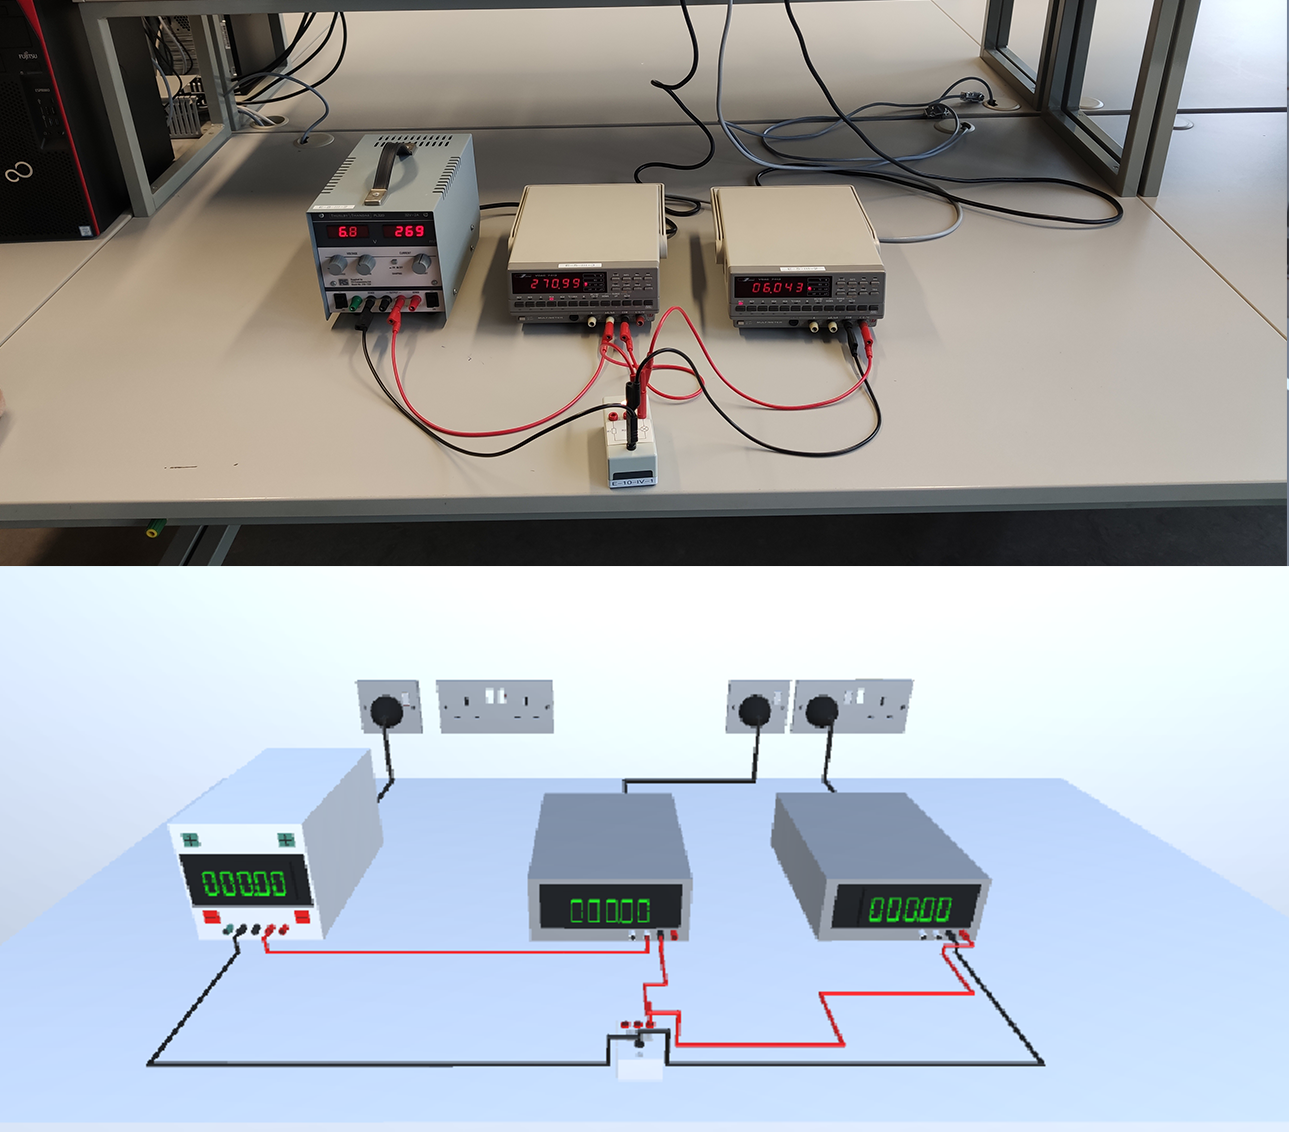
\includegraphics[width=0.95\linewidth]{etechnik_vgl}

	\end{figure}
	\vspace{20px}
\end{block}

\vspace{0.3cm}

\begin{block}{Bubblesort}
	\begin{figure}
		\centering
		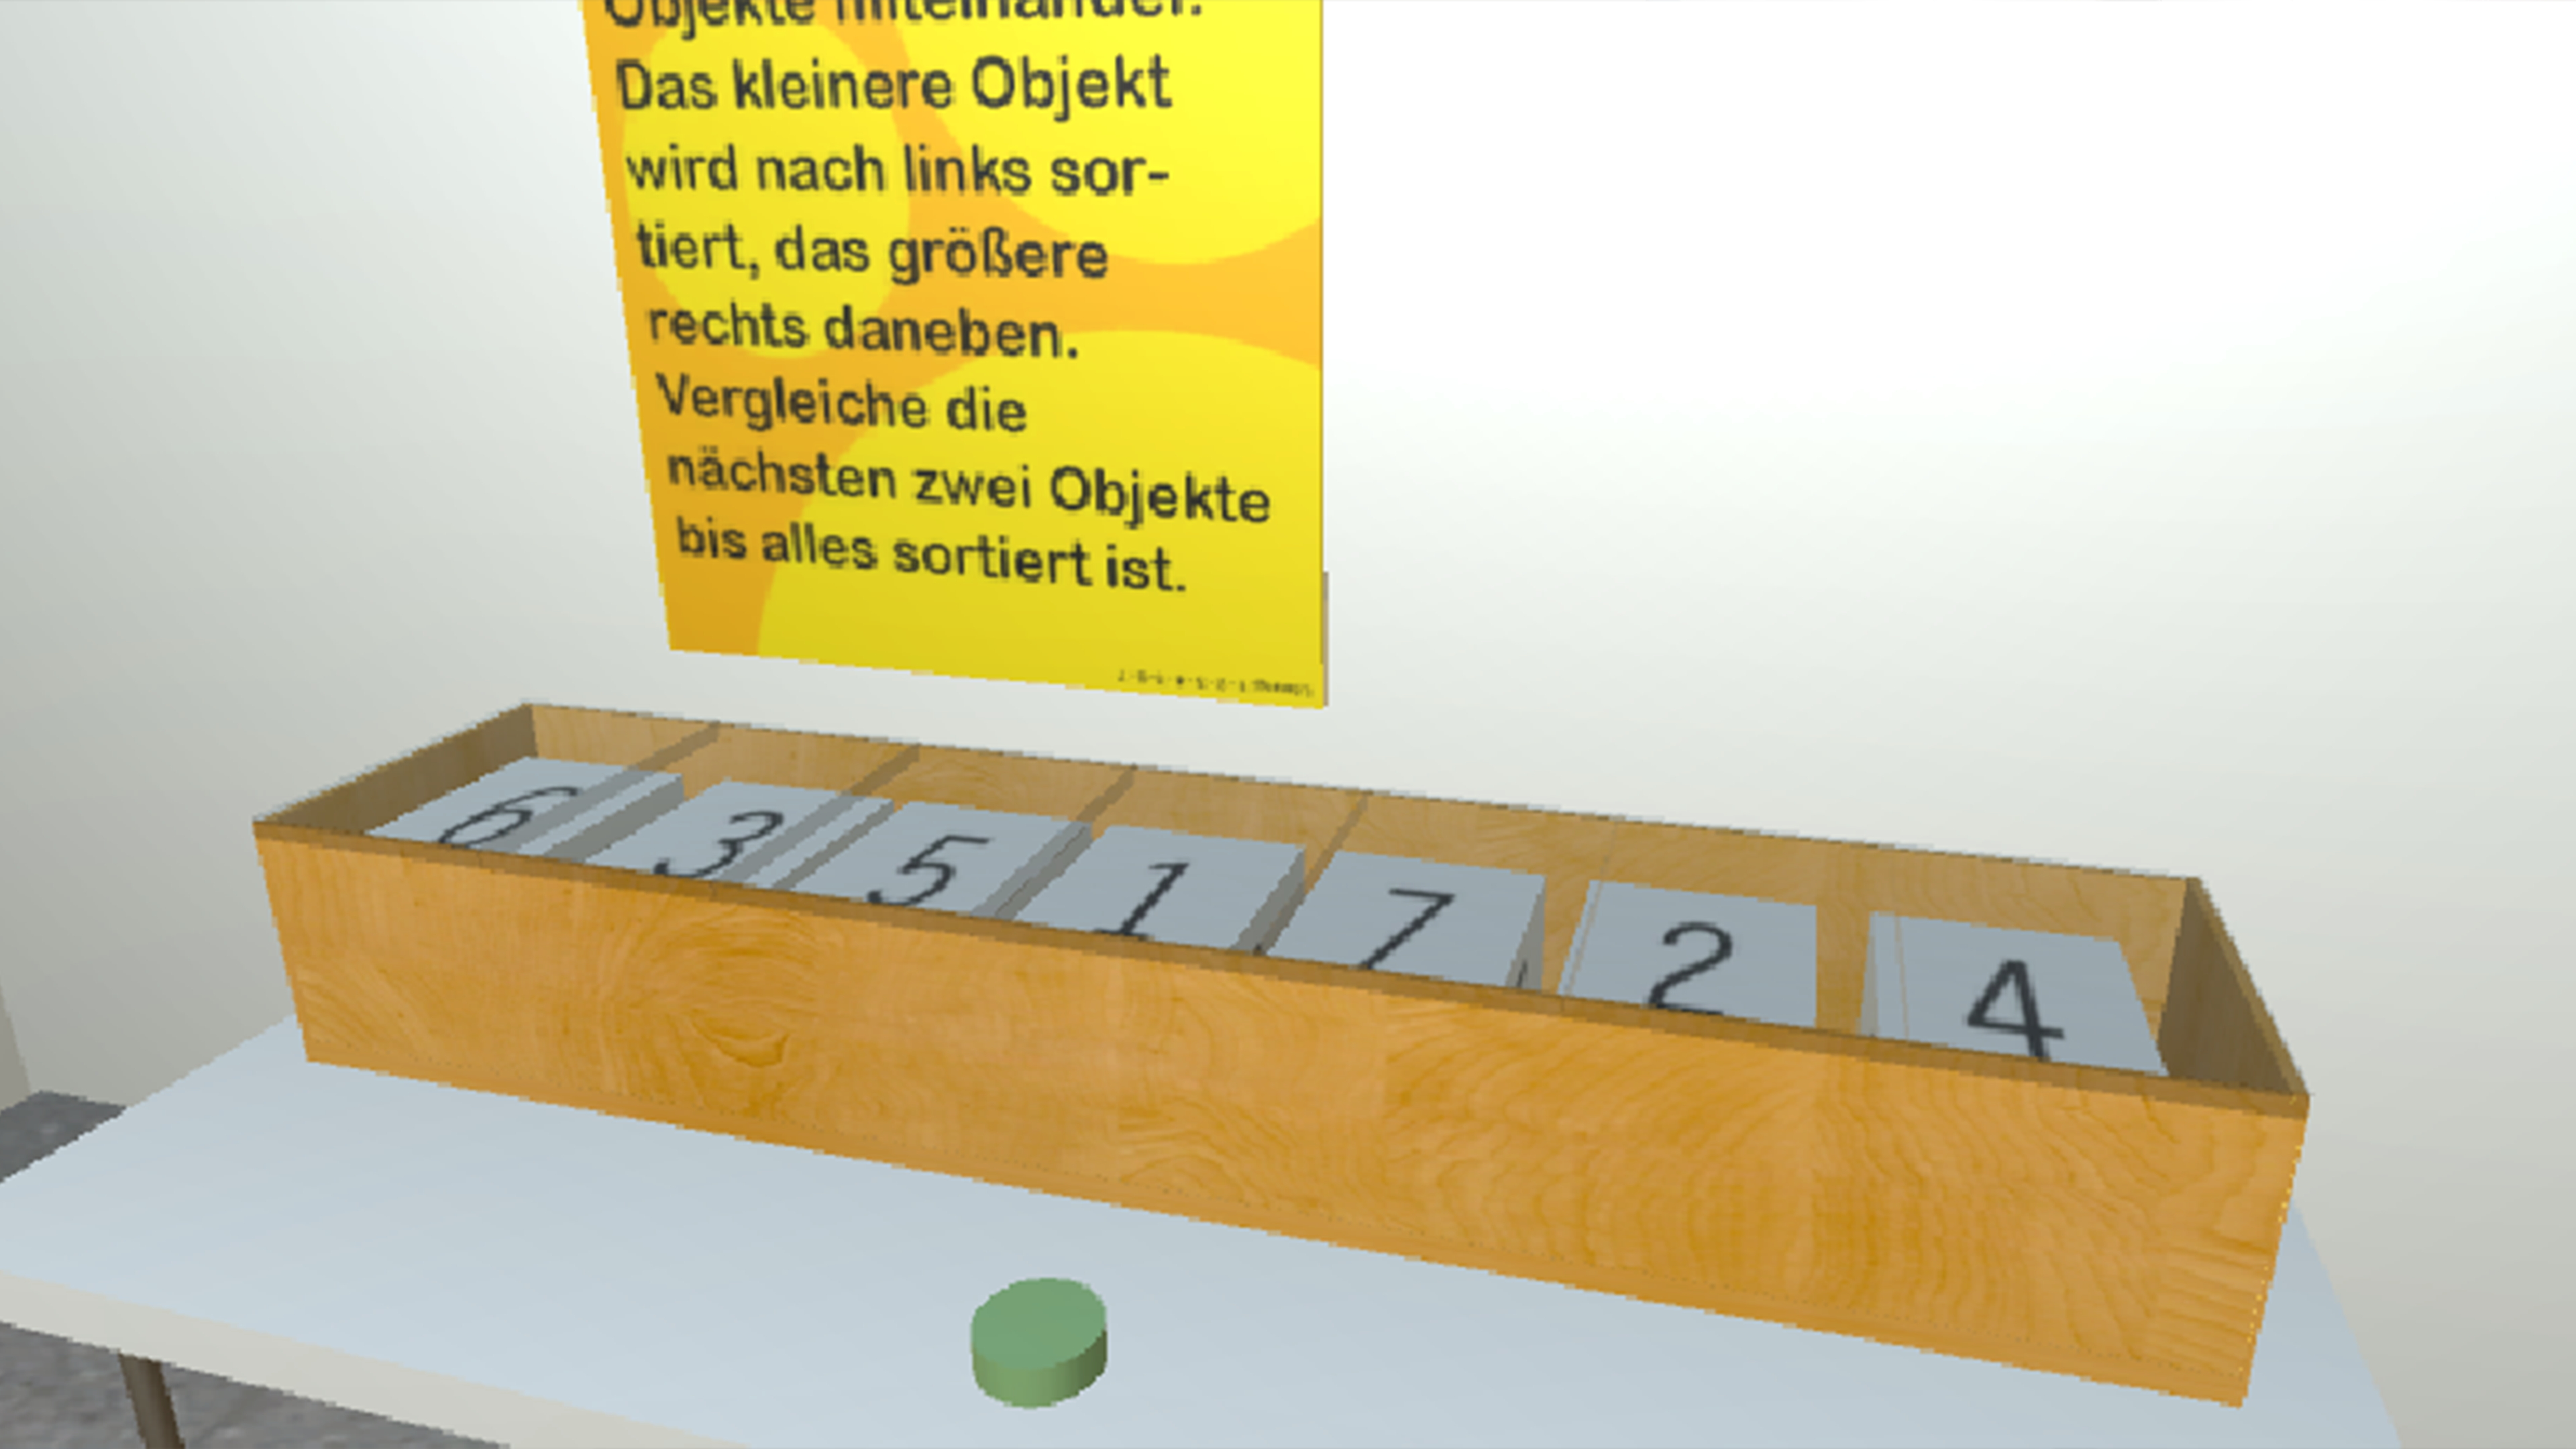
\includegraphics[width=0.95\linewidth]{informatiklab_bubblesort}

	\end{figure}
\end{block}

\vspace{0.3cm}

\begin{block}{Test}
	
	\begin{itemize}
		\item Integraler Bestandteil des persönlichen Workflows
		\item Eine weitere Anwendung auf unserem Schreibtisch
		\item Eine andere Sicht auf unsere Daten und Ergebnisse
	\end{itemize}
	\vspace{320px}
\end{block}

\vspace{0.1cm}

%----------------------------------------------------------------------------------------
\end{column} % End of the second column

\begin{column}{.015\textwidth}\end{column} % Empty spacer column

\end{columns} % End of all the columns in the poster

\begin{block}{Literatur}
	\bibliographystyle{geralpha}
	\nocite{pries:19}
	\bibliography{sample}
\end{block}

\end{frame} % End of the enclosing frame

\end{document} 